\section{Spec 8 --- Weak-label baselines}

Using just the note, we can predict the Artportalen habitat field, as well as the CrowdWater water-level class.
The dataset was split 80/10/10, stratified by platform; each CrowdWater gauge was kept in one split, which results in a 64/8/28 split for CrowdWater.
Due to EyeOnWater having no notes, we cannot predict its Forel-Ule colour field from text.
The models used were a TF-IDF with a linear SVM, and a multilingual DistilBERT~\cite{sanh2019distilbert}, with and without stopwords (Table~\ref{tab:weak}). 


\begin{table}[htbp]
\centering\small
\caption{Weak-label baselines, test macro F1 (117 habitat, 578 water-level notes).}
\label{tab:weak}
\begin{tabular}{lrr}
\toprule
Model & Habitat & Water level \\
\midrule
Majority class & 0.05 & 0.04 \\
TF-IDF + SVM & \textbf{0.73} & \textbf{0.22} \\
DistilBERT & 0.65 & 0.15 \\
\bottomrule
\end{tabular}
\end{table}

From the results, we can see that habitat is much easier to predict from the note than water level.
This is thanks to the fact that habitat is often mentioned in the note; while water level is not, since it is read from a gauge in the photo.
A surprising result is that the simple SVM had superior performance to DistilBERT, which is a much more complex model.
Removing stopwords didn't affect much the performance of the models, with the macro f1 score changing by less than 0.01 in all cases.

\section{Spec 9 --- Image--text consistency}

We compare each note against its photo with the cosine similarity of CLIP~\cite{radford2021clip} (English text) and
multilingual SigLIP~\cite{zhai2023siglip} embeddings, on 148 gold records with a photo, as well as 600 other pairs. 
Due to only 8 gold records being inconsistent, we decided to score as well each note against a different, random record's photo, 
with the expectation being that a useful model should prefer the real pair (Table~\ref{tab:clip}, Figure~\ref{fig:clip}).

\begin{table}[htbp]
\centering\small
\caption{Image--text similarity: AUC of own vs another photo, and against the gold labels.}
\label{tab:clip}
\resizebox{\columnwidth}{!}{%
\begin{tabular}{lrrrr}
\toprule
Model & Own vs other & iNaturalist & CrowdWater & Gold (consistent vs not) \\
\midrule
CLIP (English) & 0.72 & 0.80 & 0.64 & 0.73 \\
SigLIP (original) & 0.70 & 0.75 & 0.66 & 0.70 \\
SigLIP (translation) & 0.69 & 0.75 & 0.63 & 0.71 \\
\bottomrule
\end{tabular}}
\end{table}

\begin{figure}[htbp]
\centering
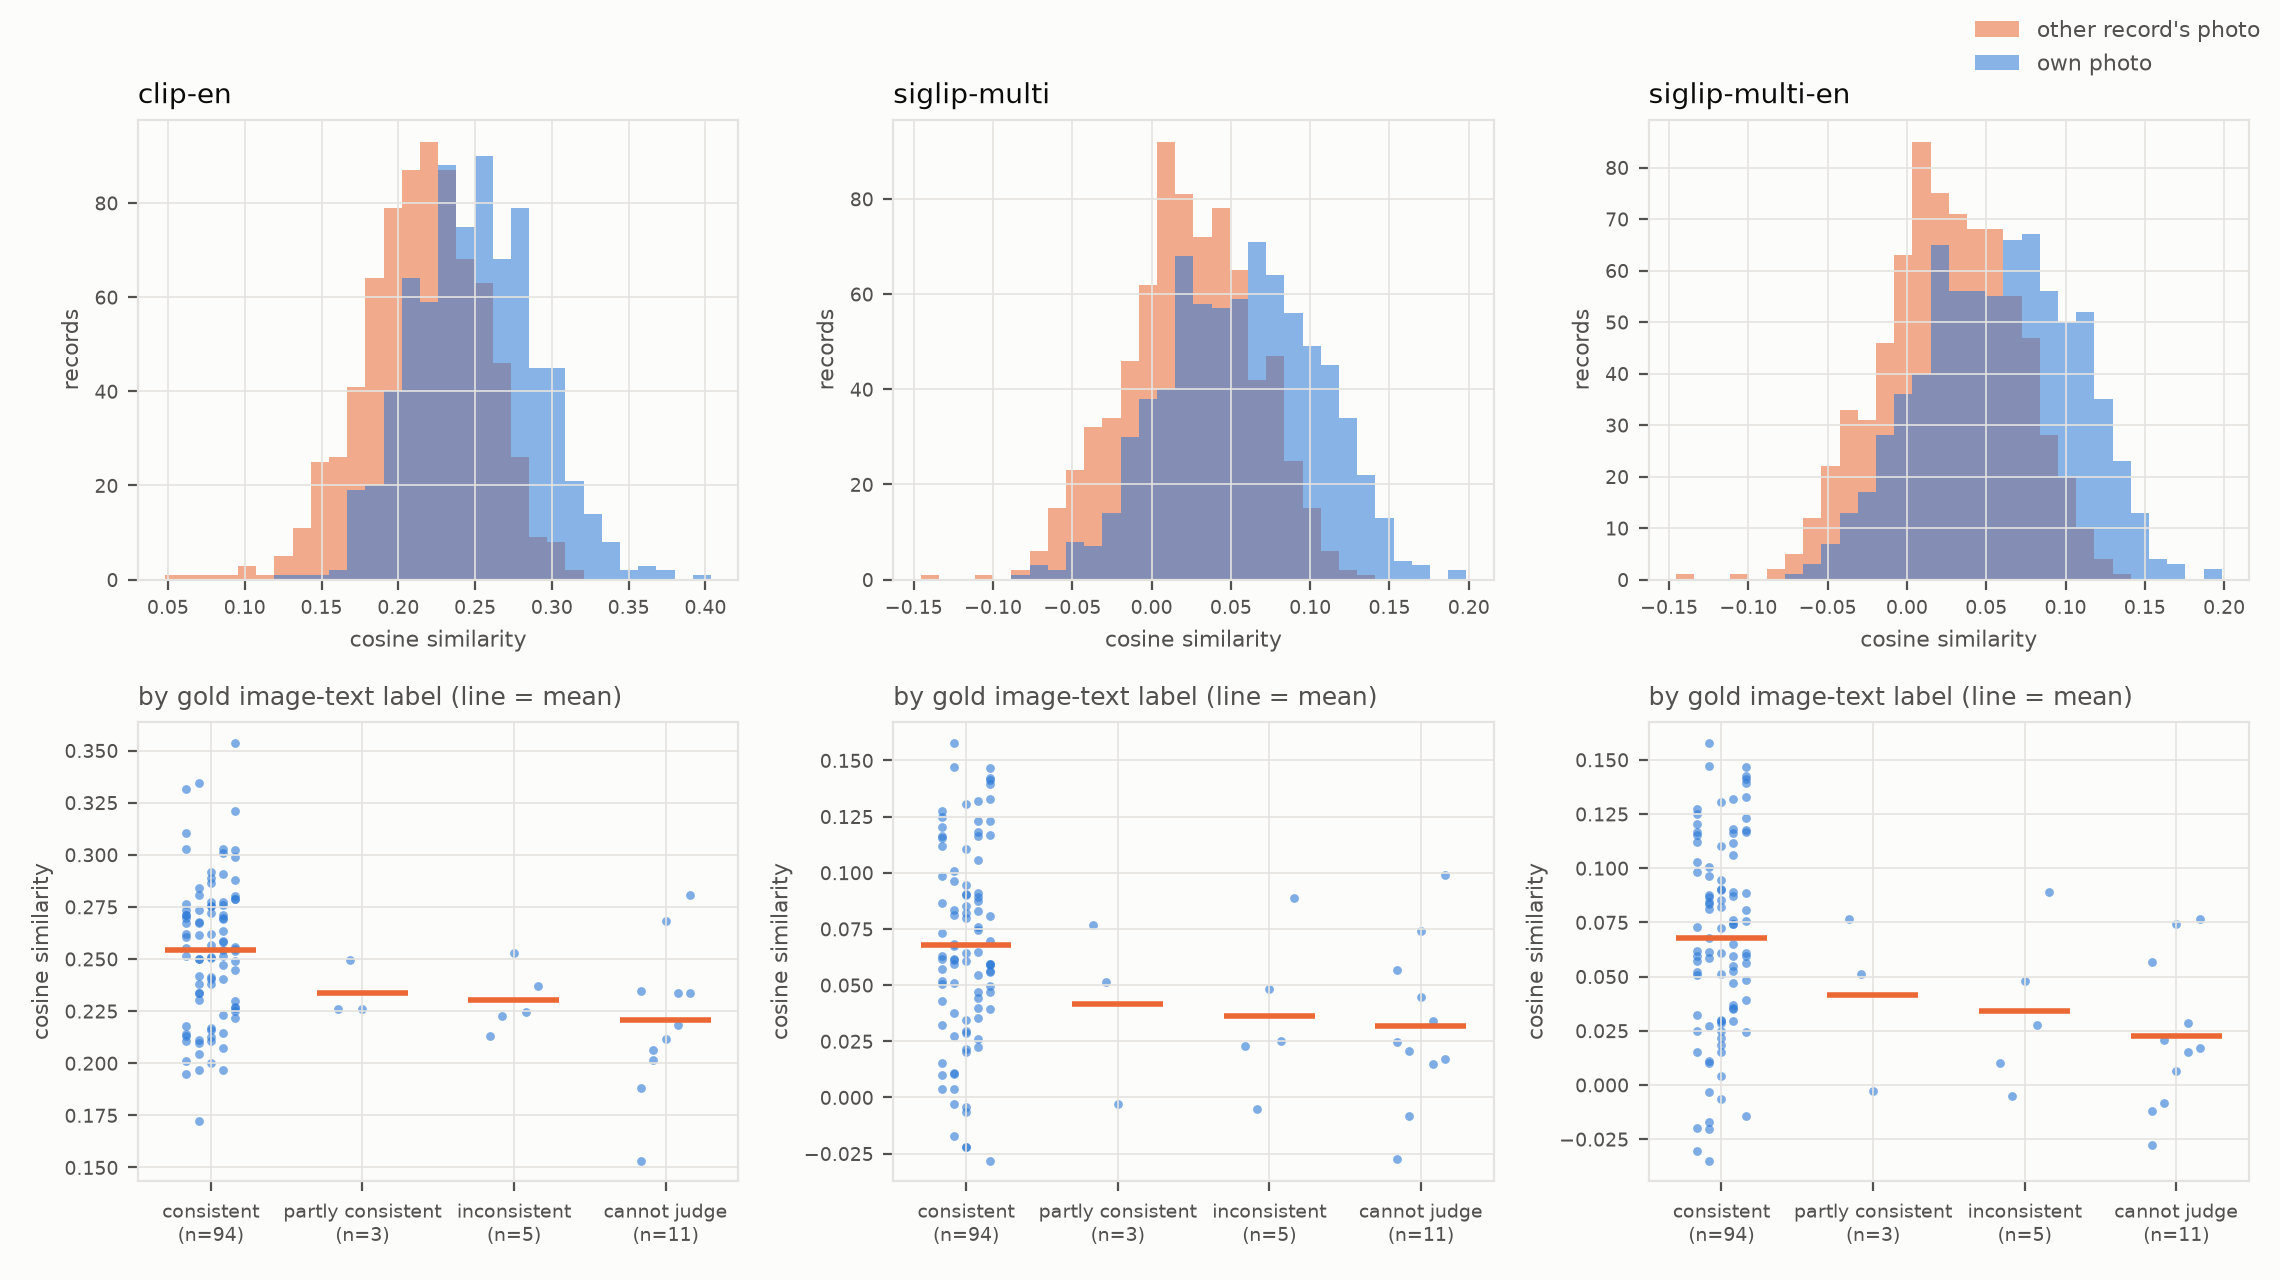
\includegraphics[width=0.85\textwidth]{spec9_similarity.png}
\caption{Similarity of a note with its own photo vs another record's photo (top) and by gold label (bottom).}
\label{fig:clip}
\end{figure}

From the results we can conclude that the real pair is preferred about 75\% of the time, which is to say about 3 times in 4.
This score is well above random chance, but it is not reliable. It works well on iNaturalist, where the note names the species in the photo,
but quite poorly on CrowdWater where all photos show a riverbank with a gauge. This is due to the fact that the models measure whether photo and note 
are about the same topic, but not whether the photo shows the condition the note describes.